\documentclass[a4paper,twoside,12pt]{article}
\usepackage[top=1.5cm,left=1.5cm,right=1.5cm,bottom=2cm]{geometry}

\usepackage[utf8]{inputenc}
\usepackage[T1]{fontenc}
\usepackage{lmodern}
\usepackage[brazilian]{babel}
\usepackage{graphicx}
%\usepackage{subfig}
\usepackage{psfrag}
\usepackage{cite}
\usepackage[cmex10]{amsmath}
\usepackage{amssymb}
\usepackage{upgreek}
\usepackage{microtype}
\usepackage{titling}
\usepackage{courier}
\usepackage[caption=false]{subfig}  % pacote para subfloats

\usepackage{url}
\usepackage{hyperref}
\hypersetup{
	colorlinks=true,
	linkcolor=blue,
	urlcolor=blue
}

% Use the 'listings' package to add code and the 'color' package to generate the highlights
\usepackage{listings}
\usepackage{color}
\definecolor{grey}{rgb}{0.6,0.6,0.6}
\definecolor{codegreen}{rgb}{0,0.6,0}
\definecolor{codegray}{rgb}{0.5,0.5,0.5}
\definecolor{codepurple}{rgb}{0.58,0,0.82}
\definecolor{backcolour}{rgb}{0.95,0.95,0.92}
\lstset{language=Python,				% set it to Python language highlighting
	backgroundcolor=\color{backcolour},
	commentstyle=\color{codegreen},
	keywordstyle=\color{magenta},
	numberstyle=\tiny\color{codegray},
	stringstyle=\color{codepurple},
	basicstyle=\ttfamily\small,		% set size of fonts
	breaklines=true,				% set automatic line breaking
	linewidth=\textwidth,			% set size of code box
	showstringspaces=false}			% show spaces as underscores only inside strings


\title{\vspace{-2cm} Processamento Digital de Sinais e Aplicações em Acústica\\ Soluções para Tutorial 04 - Quantização}
\author{\url{https://github.com/fchirono/Aulas_PDS_Acustica}}

\begin{document}
	\date{}
	\maketitle
	
	\setcounter{section}{2}
	\subsection{Função de Quantização}
	
	\begin{enumerate}
		\item Uma possível implementação da função de quantização está demonstrada abaixo:
	
\begin{lstlisting}[frame=single]

def quantizar_sinal(sinal, n_bits, v_max=1.0):
	"""
	Quantizar um sinal de tensao usando "Linear Pulse-Code Modulation"
	(L-PCM) com 'n_bits', e quantizador do tipo "midtread".
	
	Parametros:
	-----------
	sinal : array-like
	Sinal de tensao a ser quantizado
	
	n_bits : int
	Numero de bits utilizado na quantizacao
	
	v_max : float, opcional
	Tensao maxima de entrada do conversor AD (padrao: 1.0V)
	
	Retorna:
	--------
	Tupla contendo:
	- sinal_quantizado: sinal de tensao com amplitudes quantizadas
	- erro: sinal de erro (diferenca) entre sinal original e quantizado
	- tamanho_nivel: tamanho de cada nivel de quantizacao, em volts
	"""
	
	# Converter argumento de entrada em array numpy
	sinal_tensao = np.array(sinal)
	
	# Calcular numero de niveis do conversor
	#   --> um bit eh utilizado para armazenar o sinal (+ ou -)
	n_niveis = 2**(n_bits-1)
	
	# tensao minima de entrada do conversor AD (bipolar)
	v_min = -v_max
	
	# Calcular tamanho de cada nivel binario
	tamanho_nivel = (v_max - v_min) / n_niveis
	
	# Criar array com os diferentes niveis de tensao eletrica
	# usando 'n_niveis' de '-v_max' ate (mas nao incluindo) '+v_max'
	niveis_tensao = np.linspace(v_min, v_max, n_niveis, endpoint=False)
	
	# Limitar o sinal para a faixa de tensao especificada
	#   --> O valor maximo deve ser um nivel abaixo de '+v_max'
	sinal_limitado = np.clip(sinal_tensao, v_min, v_max - tamanho_nivel)
	
	# Calcula o sinal quantizado usando um quantizador tipo "midtread"
	# (Lipshitz et al, 1992)
	sinal_quantizado = tamanho_nivel * np.floor(sinal_limitado/tamanho_nivel + 1/2)
	
	# Calcular o erro de quantizacao
	erro_quantizacao = sinal_tensao - sinal_quantizado
	
	return sinal_quantizado, erro_quantizacao, tamanho_nivel

\end{lstlisting}  
	
		\item A amostragem de um sinal senoidal com as características dadas no Exercício 2.1.2 está demonstrada na Figura \ref{fig:Ex_2_1_2}. Nota-se que o sinal de erro tem amplitude comparável ao sinal de entrada, indicando que será perceptível. O sinal de erro também é periódico e com o mesmo período do sinal de entrada, indicando que terá características tonais.
		
		\begin{figure}[h]
			\centering
			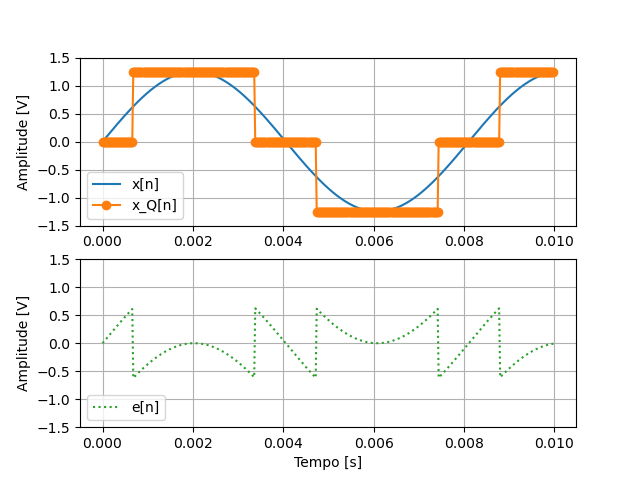
\includegraphics[width=0.75\textwidth]{2_1_SinalQuantizadoTempo_4bits.png}
			\caption{Sinal senoidal original $x[n]$, sinal quantizado $x_Q[n]$, e sinal de erro $e[n]$ para quantizador do Exercício 2.1.2.}
			\label{fig:Ex_2_1_2}
		\end{figure}
		
		
		\item A densidade espectral de potência dos sinais original, quantizado e de erro estão demonstradas na Figura \ref{fig:Ex_2_1_3}. O sinal original apresenta apenas um pico apenas na sua frequência fundamental de 123,4 Hz, enquanto o sinal quantizado apresenta uma série de outros picos de amplitudes decrescentes. Claramente, o sinal quantizado não é uma boa representação do sinal original devido a estes picos adicionais. Os picos no espectro do sinal de erro - assim como no espectro do sinal quantizado - estão distribuídos de forma regular por uma banda larga de frequências.
		
		\begin{figure}[h]
			\centering
			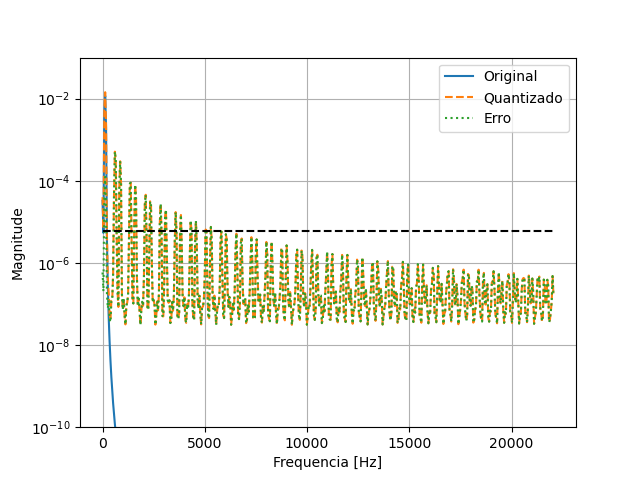
\includegraphics[width=0.75\textwidth]{2_1_SinalQuantizadoPSD_4bits.png}
			\caption{Densidade Espectral de Potência dos sinal senoidal original, sinal quantizado, e sinal de erro. A densidade espectral teórica do sinal de erro (Eq. 5) está indicada pela linha preta tracejada. }
			\label{fig:Ex_2_1_3}
		\end{figure}
		
		\item A densidade espectral teórica do sinal de erro (Eq. 5) está indicada na Figura \ref{fig:Ex_2_1_3} pela linha preta tracejada. O valor teórico não é uma boa aproximação para a densidade espectral do sinal do erro para este caso em particular.
		
		\item Ao auralizar os sinais, nota-se que o sinal quantizado apresenta níveis grosseiros de distorção claramente audíveis, e não é uma boa aproximação do sinal original. Apesar do sinal original possuir apenas uma frequência (123,4 Hz), o sinal quantizado claramente possui frequências mais altas presentes, conforme sugerido pelos vários picos no seu espectro em frequência.
		
		\item Repetindo o exercício:
		
		\begin{itemize}
			\item $N_{bits}=8$: A Figura \ref{fig:Ex_2_1_8bits} mostra os sinais no tempo e suas densidades espectrais na frequência. Nota-se que o sinal quantizado agora se aproxima bem do sinal original, resultando em um sinal de erro de baixa amplitude. No domínio da frequência, o sinal quantizado ainda apresenta picos adicionais distribuídos em uma banda larga de frequências, mas estes apresentam estrutura menos regular e valores mais próximos da densidade espectral de erro teórica. Ao auralizar os sinais, os efeitos de quantização soam menos como uma distorção grosseira do sinal de entrada e mais como um pequeno ruído de fundo.
			
			\begin{figure}[h]
				\centering
				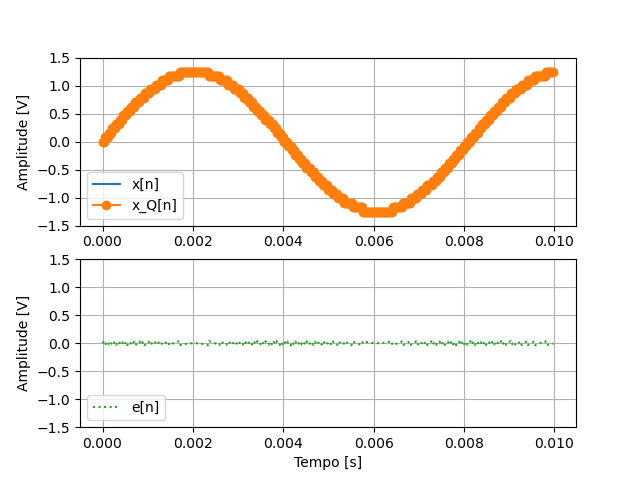
\includegraphics[width=0.49\textwidth]{2_1_SinalQuantizadoTempo_8bits.png}
				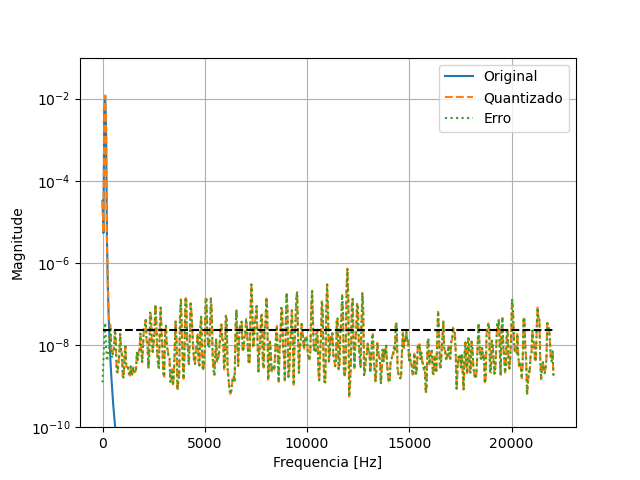
\includegraphics[width=0.49\textwidth]{2_1_SinalQuantizadoPSD_8bits.png}
				\caption{Repetição do Exercício 2.1 com $N_{bits}=8$.}
				\label{fig:Ex_2_1_8bits}
			\end{figure}
			
			\item $N_{bits}=16$: A Figura \ref{fig:Ex_2_1_16bits} mostra os sinais no tempo e suas densidades espectrais na frequência. As diferenças entre os sinais original e quantizado não são mais visíveis na Figura. O espectro do sinal quantizado agora se assemelha muito mais ao espectro do sinal original, e não possui mais picos visíveis. Porém, este apresenta um resíduo de valor quase uniforme distribuído por todas as frequências, que coincide com a densidade espectral de erro teórica - note que esta apresenta um valor muito mais baixo que nos casos anteriores. Os sinais auralizados soam idênticos, sem qualquer diferença perceptível - note que 16 bits é um valor típico utilizado na distribuição de áudio digital por CDs e diversas plataformas de \emph{streaming}.
			
			\begin{figure}[h]
				\centering
				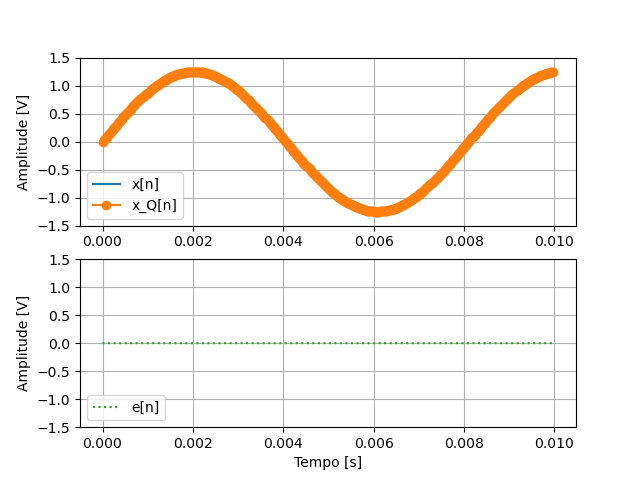
\includegraphics[width=0.49\textwidth]{2_1_SinalQuantizadoTempo_16bits.png}
				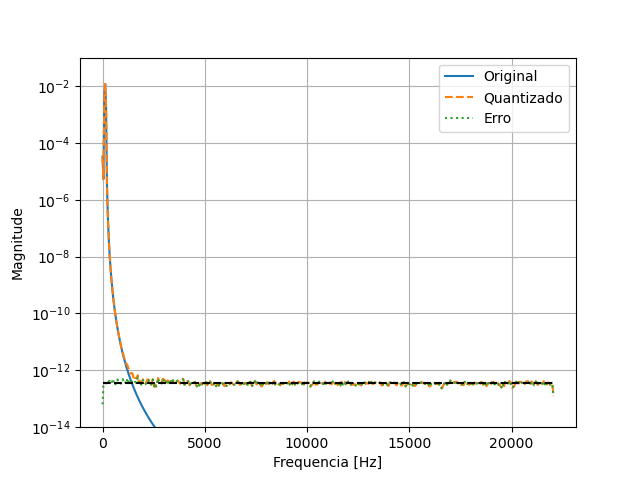
\includegraphics[width=0.49\textwidth]{2_1_SinalQuantizadoPSD_16bits.png}
				\caption{Repetição do Exercício 2.1 com $N_{bits}=16$.}
				\label{fig:Ex_2_1_16bits}
			\end{figure}
		\end{itemize}
		
	\end{enumerate}
	
	\subsection{Amplitude do Sinal e Saturação}
	
	\begin{enumerate}
		\item A Figura \ref{fig:Ex_2_1_10V_4bits} mostra os sinais no tempo e e frequência para o caso $V_0=10$ V. Nota-se aqui que o sinal de entrada possui amplitude maior que o nível de tensão máxima do conversor, resultando no ``ceifamento'' (\emph{clipping}, em inglês) dos picos do sinal senoidal, um sinal de erro que apresenta grande magnitude e estrutura periódica, e em um sinal quantizado que se assemelha a uma onda quadrada. Novamente, tem-se que o sinal quantizado apresenta distorção grosseira e audível, com picos distribuídos de forma regular por todas as frequências.
		
		\begin{figure}[h]
			\centering
			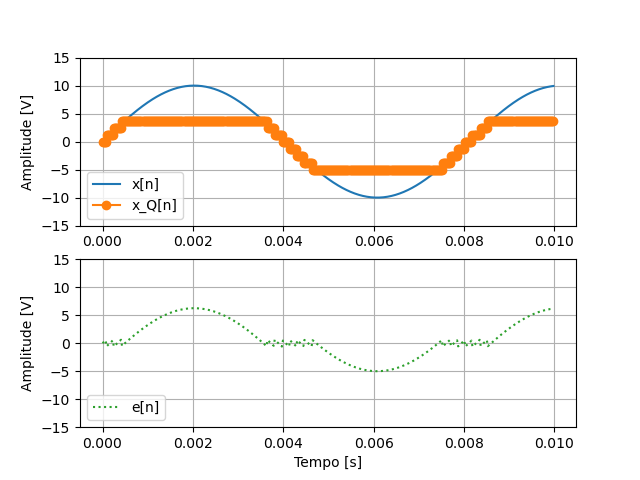
\includegraphics[width=0.49\textwidth]{2_1_SinalQuantizadoTempo_10V_4bits.png}
			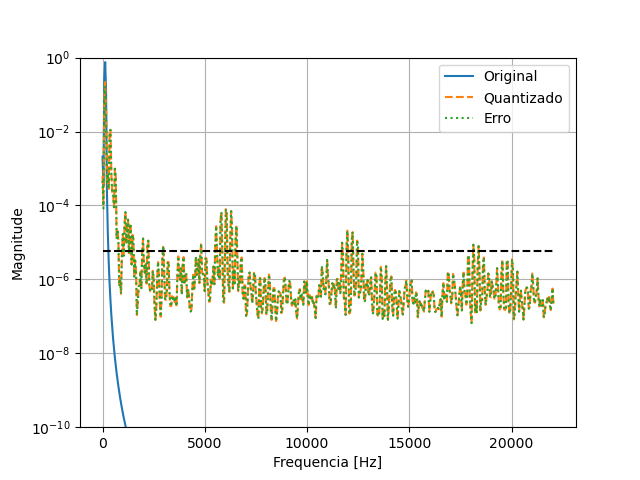
\includegraphics[width=0.49\textwidth]{2_1_SinalQuantizadoPSD_10V_4bits.png}
			\caption{Repetição do Exercício 2.1 com $V_0 = 10$ V e $N_{bits}=4$.}
			\label{fig:Ex_2_1_10V_4bits}
		\end{figure}
		
		\item A Figura \ref{fig:Ex_2_1_05V_4bits} mostra os sinais no tempo e e frequência para o caso $V_0=0.5$ V. Desta vez, o sinal de entrada apresenta amplitude menor que o LSB do conversor (neste caso, $\Delta v = 1.25$ V), e portanto nenhuma amostra é adquirida com sucesso. O sinal quantizado apresenta valor zero em todas as suas amostras, e obviamente não é uma representação correta do sinal original. 
		
		\begin{figure}[h]
			\centering
			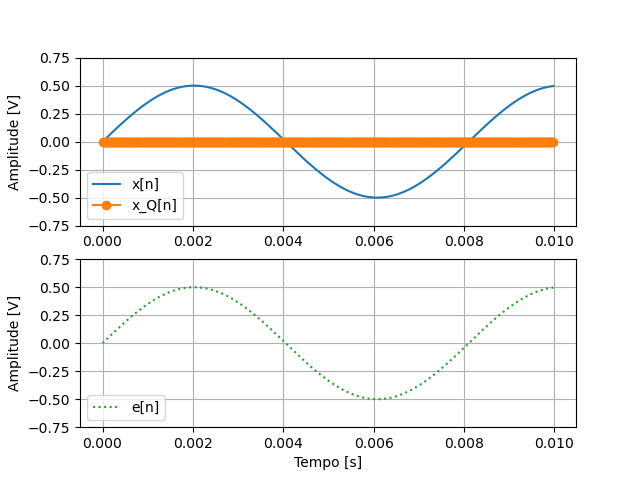
\includegraphics[width=0.49\textwidth]{2_1_SinalQuantizadoTempo_0.5V_4bits.png}
			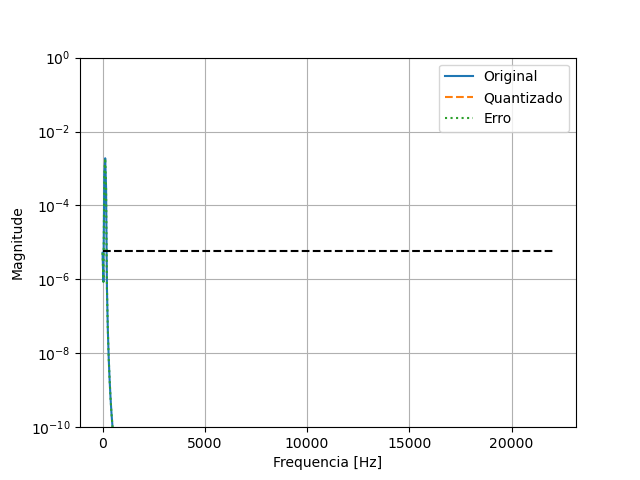
\includegraphics[width=0.49\textwidth]{2_1_SinalQuantizadoPSD_0.5V_4bits.png}
			\caption{Repetição do Exercício 2.1 com $V_0 = 0.5$ V e $N_{bits}=4$.}
			\label{fig:Ex_2_1_05V_4bits}
		\end{figure}
	\end{enumerate}
	
	\clearpage
	\newpage
	\subsection{\emph{Dithering} (OPCIONAL)}
	
		\begin{enumerate}
		\item Uma possível implementação da função de quantização com dithering está demonstrada abaixo:
		
\begin{lstlisting}[frame=single]	
def quantizar_sinal_dither(sinal, n_bits, v_max=1.0, dither=False):
	"""
	Quantizar um sinal de tensao usando "Linear Pulse-Code Modulation" (L-PCM)
	com 'n_bits', e quantizador do tipo "midtread".
	
	Parametros:
	-----------
	sinal : array-like
		Sinal de tensao a ser quantizado
	
	n_bits : int
		Numero de bits utilizado na quantizacao
	
	v_max : float, opcional
		Tensao maxima de entrada do conversor AD (padrao: 1.0V)
	
	dither : bool, opcional
		Flag para aplicar dithering triangular ao sinal de entrada
	
	Retorna:
	--------
	Tupla contendo:
	- sinal_quantizado: sinal de tensao com amplitudes quantizadas
	- erro: sinal de erro (diferenca) entre sinal original e quantizado
	- tamanho_nivel: tamanho de cada nivel de quantizacao, em volts
	"""
	
	# Converter argumento de entrada em array numpy
	sinal_tensao = np.array(sinal)
	
	# Calcular numero de niveis do conversor
	#   --> um bit eh utilizado para armazenar o sinal (+ ou -)
	n_niveis = 2**(n_bits-1)
	
	# tensao minima de entrada do conversor AD (bipolar)
	v_min = -v_max
	
	# Calcular tamanho de cada nivel binario
	tamanho_nivel = (v_max - v_min) / n_niveis
	
	if dither:
		# dithering de espectro triangular, amplitude 2-LSB pico-a-pico
		#  --> soma de dois ruidos de espectro retangular independentes
		ruido1 = rng.uniform(low = -tamanho_nivel,
					high = +tamanho_nivel,
					size = t.shape[0])
		ruido2 = rng.uniform(low = -tamanho_nivel,
					high = +tamanho_nivel,
					size = t.shape[0])
		ruido = (ruido1 + ruido2)/2
		
		# adicionar o ruido ao sinal original
		sinal_tensao += ruido
		
		# # plotar histograma do ruido de dithering para confirmar
		# # a distribuicao triangular
		# plt.figure()
		# plt.hist(ruido, bins=100)
	
	# Criar array com os diferentes niveis de tensao eletrica
	# usando 'n_niveis' de '-v_max' ate (mas nao incluindo) '+v_max'
	niveis_tensao = np.linspace(v_min, v_max, n_niveis, endpoint=False)
	
	# Limitar o sinal para a faixa de tensao especificada
	#   --> O valor maximo deve ser um nivel abaixo de '+v_max'
	sinal_limitado = np.clip(sinal_tensao, v_min, v_max - tamanho_nivel)
	
	# Calcula o sinal quantizado usando um quantizador tipo "midtread"
	# (Lipshitz et al, 1992)
	sinal_quantizado = tamanho_nivel * np.floor(sinal_limitado/tamanho_nivel + 1/2)
	
	# Calcular o erro de quantizacao
	erro_quantizacao = sinal_tensao - sinal_quantizado
	
	return sinal_quantizado, erro_quantizacao, tamanho_nivel

\end{lstlisting}  
	
		\item A Figura \ref{fig:Ex_2_1_05V_4bits} mostra os sinais no tempo e e frequência para o caso com \emph{dithering}. Nota-se que o sinal quantizado agora apresenta amostras com valores acima e abaixo do sinal original de forma aleatória, resultando em um sinal de erro com características não determinísticas.
		
		\item O espectro do erro com \emph{dithering} apresenta valor quase constante em frequência, sem apresentar picos ou outras características regulares, se assemelhando a ruído branco. Como resultado, o \emph{dithering} mascara as distorções determinísticas do sinal quantizado, mas a adição de ruído é perceptível como um aumento no ruído de fundo.
		
		\item Ao auralizar o sinal quantizado com \emph{dithering} deste exemplo, ouve-se o sinal tonal original sem características de ``distorção'', mas nota-se um ruído de fundo bem pronunciado. Nota-se que o exemplo apresentado aqui exagera este efeito para fins didáticos; em casos reais estes efeitos não são tão óbvios, e tipicamente ruído de fundo com características de ruído branco tende a ser menos ``ofensivo'' para a maioria das pessoas do que distorção determinística. Repetir o exercício usando um número maior de bits por amostra resultará em efeitos mais sutis, mais próximos aos observados em conversores reais.
		
		\begin{figure}[h]
			\centering
			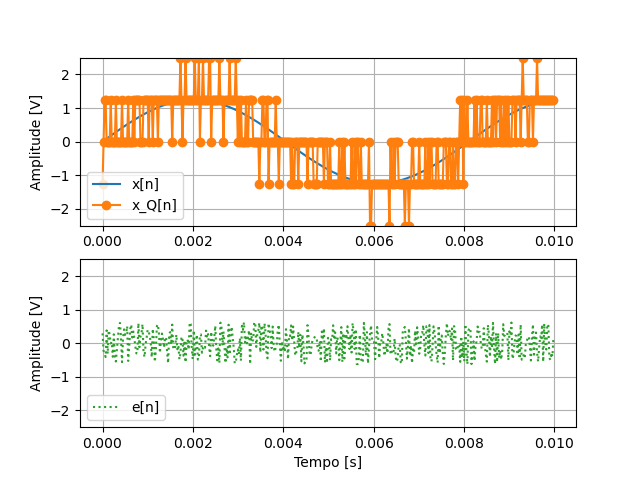
\includegraphics[width=0.49\textwidth]{2_1_SinalQuantizadoTempo_1.25V_4bits_dither.png}
			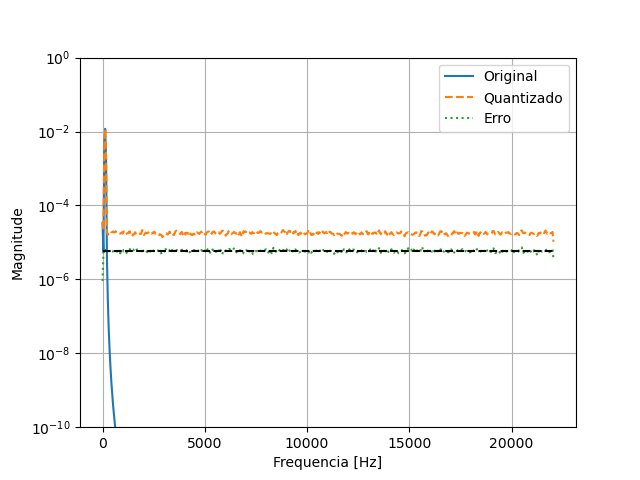
\includegraphics[width=0.49\textwidth]{2_1_SinalQuantizadoPSD_1.25V_4bits_dither.png}
			\caption{Repetição do Exercício 2.1 com $V_0 = 1.25$ V e $N_{bits}=4$, com \emph{dithering}.}
			\label{fig:Ex_2_1_125V_4bits_dithering}
		\end{figure}
	\end{enumerate}
\end{document}
